%!TEX TS-program = xelatex
%!TEX encoding = UTF-8 Unicode

\documentclass[tikz,border=1]{standalone}
\usetikzlibrary{positioning}

\begin{document}
  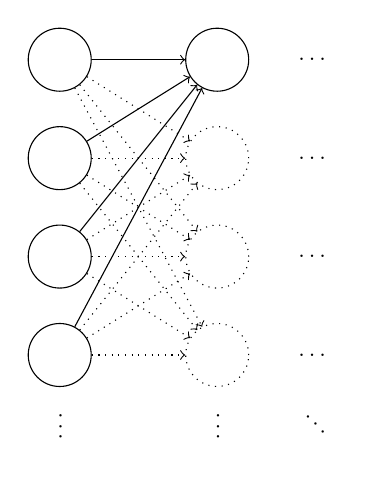
\begin{tikzpicture}[
    neuron/.style={circle,draw,inner sep=0pt,minimum size=8mm},
    font=\footnotesize
    ]

    % left layers:
    \foreach \y in {0,...,3}
      \node (l\y) at (0, \y * 1.25 + 1 * 1.25) [neuron] {};

    % right layers:
    \foreach \y in {0,...,2}
      \node (r\y) at (2, \y * 1.25 + 1 * 1.25) [neuron,dotted] {};
      
    \node (r3) at (2, 3 * 1.25 + 1.25) [neuron] {};

    % right text:
    \foreach \y in {0,...,3}
      \node (tr\y) [right=0.5 of r\y] {$\ldots$};

    % bottom text:
    \node [below=0.5 of l0,rotate=-90,yshift=1.5mm] {$\ldots$};
    \node [below=0.5 of r0,rotate=-90,yshift=1.5mm] {$\ldots$};
    \node [below=0.5 of tr0,rotate=-45,xshift=2mm] {$\ldots$};
    
    \foreach \x in {0,...,3}
        \draw [->] (l\x) to (r3);

    \foreach \x in {0,...,3}
      \foreach \y in {0,...,2}
        \draw [dotted,->] (l\x) to (r\y);
        
    % \draw[->] (r0) -- ++(1,0);
    % \draw[->] (r1) -- ++(1,0);

  \end{tikzpicture} 
\end{document}
